\section*{Теоретическая часть:}
\begin{enumerate}
    \item Гониометр служит для точного измерения углов.  
    
    \item Показатель преломления призмы. \\
    \begin{figure}[h!]
        \noindent\centering{
            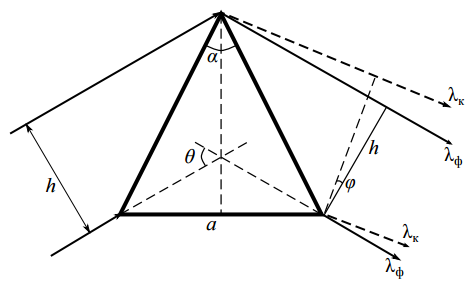
\includegraphics[height = 4cm]{1.png}
        }
        \caption{Призма.}
    \end{figure} \\
%    \newpage
    Минимальное отклонение луча, преломленного призмой, от направления луча, падающего на призму, получается при симметричном ходе луча
    ($\delta$ --- угол минимального отклонения, $\alpha$ --- преломляющий угол, $n$ --- показатель преломления): \\
    \begin{align}
        n = \frac{\sin{\frac{\alpha + \delta}{2}}}{\sin{\frac{\alpha}{2}}}
    \end{align} 
    
    \item Дисперсионная кривая --- график зависимости $n(\lambda)$ \\
        \begin{enumerate}
            \item средняя дисперсия: $D = n_F - n_C$
            \item коэффициент диспрсии: $\nu = \frac{n_D - 1}{n_F - n_C}$, где:
        \end{enumerate}
    $n_D$ --- показатель преломления для $\lambda_D = 589,3nm$ (среднее значения длин волн желтого дуплета натрия) \\
    $n_F$ --- показатель преломления для $\lambda_F = 486,1nm$ (голубая линия водорода) \\
    $n_C$ --- показатель преломления для $\lambda_C = 656,3nm$ (красная линия водорода) \\
    
    \item Разрешающая способность призмы: $R = \frac{\lambda}{\delta\lambda} = b \frac{dn}{d\lambda}$ \\
    $\delta\lambda$ --- минимальный интервал длин волн, разрешаемый по критерию Релея \\
    $b$ --- размер основания призмы, если вся рабочая грань призмы освещена параллельным пучком 
    
    \item Принцип Гюйгенса-Френеля:
    каждый элемент волнового фронта можно рассматривать как центр вторичных возмущений,
    порождающего вторичные сферические волны, а результирующее световое поле в каждой точке пространства
    будет определяться интерференцией этих волн. \\
    Дисперсия --- явления, обусловленные зависимостью абсолютного показателя преломления вещества от частоты света.
%    \item Получение эллиптически поляризованного света. \\
%    \begin{figure}[h!]
%        \noindent\centering{
%            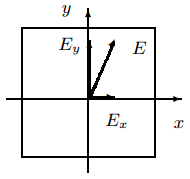
\includegraphics[height = 4cm]{Selection_048.png}
%        }
%        \caption{Разложение линейно поляризованного света по главным направлениям двоякопреломляющей пластинки.}
%    \end{figure} \\
    
\end{enumerate}